%!TEX root = ../../../adrien_gomar_phd.tex

\subsection{Convergence of the computations} % (fold)
\label{sub:dream_convergence}

\begin{figure}[htb]
  \centering
  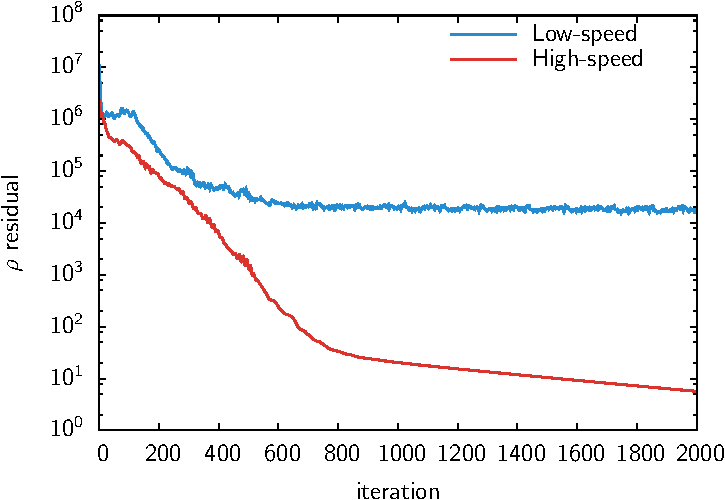
\includegraphics[width=.4\textwidth]{DREAM_RESIDUALS_PPT.pdf}
  \caption{Convergence of the steady computations.}
  \label{fig:dream_operating_point}
\end{figure}

\subsection{Operating point} % (fold)
\label{sub:dream_operating_point}

\begin{figure}[htb]
  \centering
  \subfigure[$C_p$]{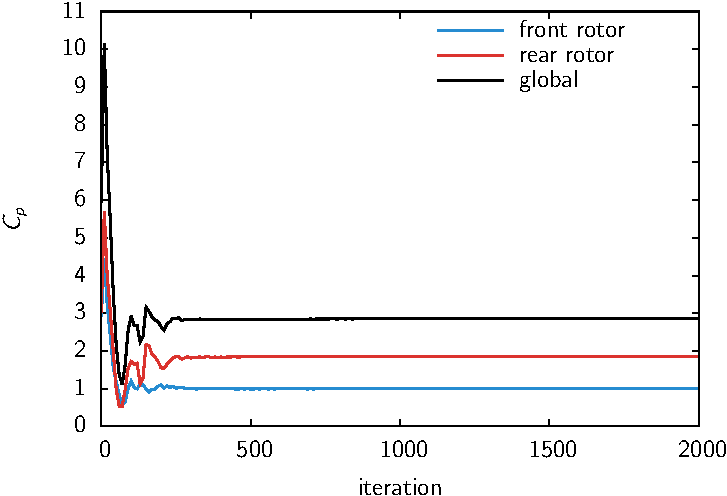
\includegraphics[width=.32\textwidth]{DREAM_LS_FORCES_CP_PPT.pdf}}
  \subfigure[$C_t$]{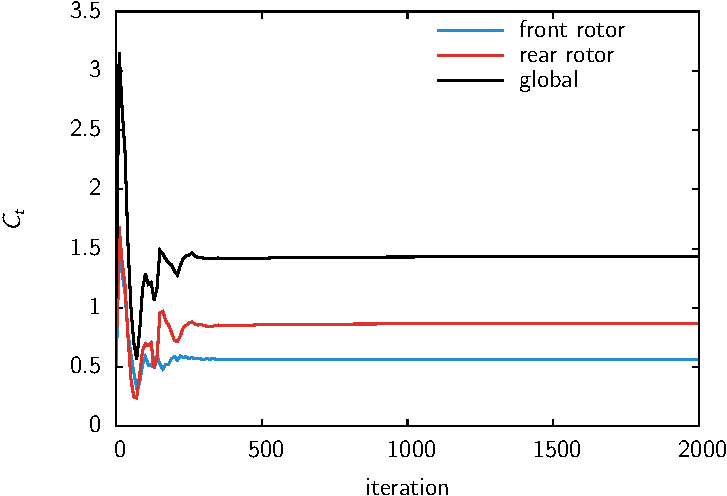
\includegraphics[width=.32\textwidth]{DREAM_LS_FORCES_CT_PPT.pdf}}
  \subfigure[$\eta$]{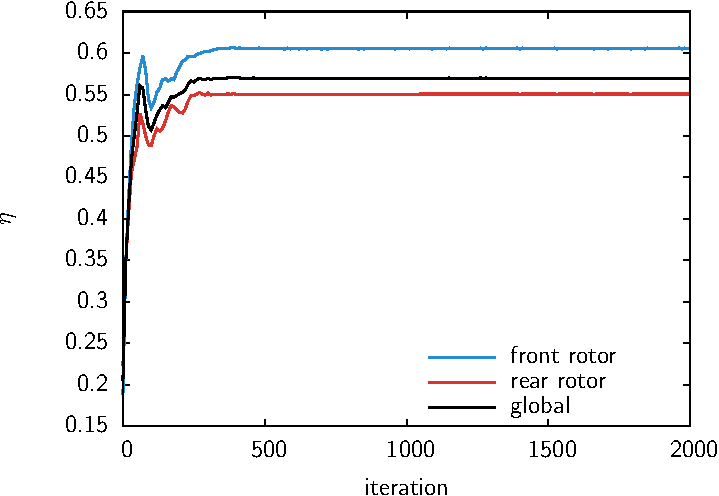
\includegraphics[width=.32\textwidth]{DREAM_LS_FORCES_ETA_PPT.pdf}}
  \caption{Convergence of the steady low-speed similarity coefficients.}
  \label{fig:dream_ls_operating_point}
\end{figure}

\begin{figure}[htb]
  \centering
  \subfigure[$C_p$]{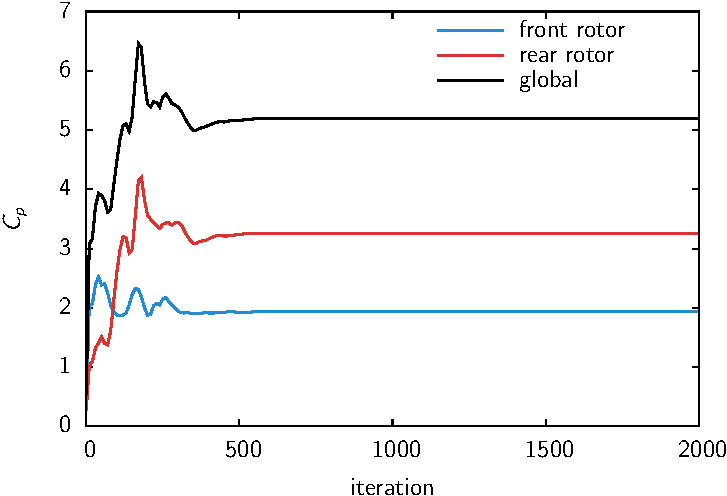
\includegraphics[width=.32\textwidth]{DREAM_HS_FORCES_CP_PPT.pdf}}
  \subfigure[$C_t$]{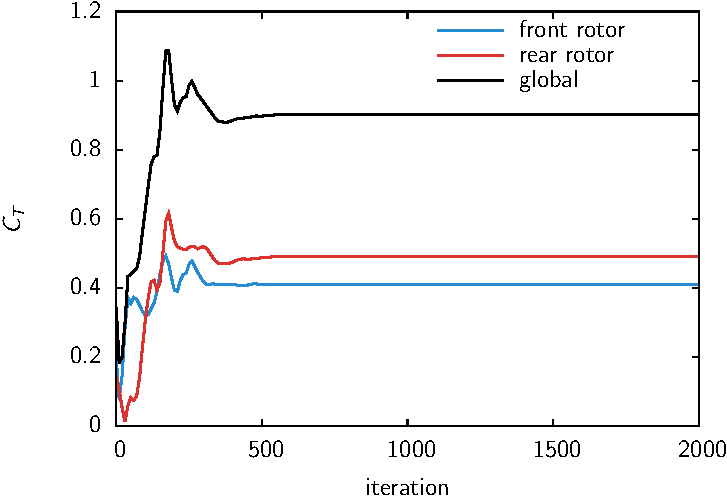
\includegraphics[width=.32\textwidth]{DREAM_HS_FORCES_CT_PPT.pdf}}
  \subfigure[$\eta$]{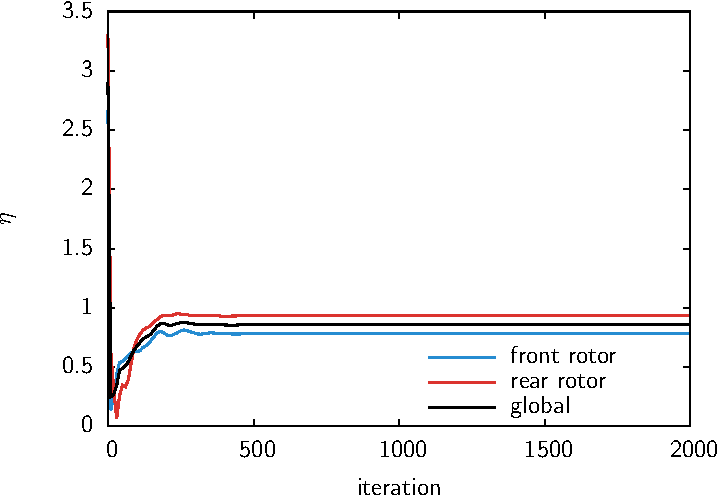
\includegraphics[width=.32\textwidth]{DREAM_HS_FORCES_ETA_PPT.pdf}}
  \caption{Convergence of the steady high-speed similarity coefficients.}
  \label{fig:dream_hs_operating_point}
\end{figure}

\begin{table}[htbp]
  \ra{1.3} \centering
  \begin{tabular}{lccc}
    \toprule
    \phantom{abdefghijk}& $C_t$ & $C_p$ & $\eta$ \\
    \midrule
    Take-off & $0.2$ & $5739~\textrm{tr.min-1}$ & 1.06 \\
    Cruise & $0.73$ & $6057~\textrm{tr.min-1}$ & 3.7 \\
    \bottomrule
  \end{tabular}
  \caption{Flight condition parameters.}
  \label{tab:dream_flight_condition}
\end{table} 


\subsection{Flow field around the blades} % (fold)
\label{sub:dream_flow_field}

\subsection{Radial profiles} % (fold)
\label{sub:dream_radial_profiles}